% !TEX TS-program = pdflatexmk
\documentclass[12pt]{article}

% Layout.
\usepackage[top=1in, bottom=0.75in, left=1in, right=1in, headheight=1in, headsep=6pt]{geometry}

% Fonts.
\usepackage{mathptmx}
\usepackage[scaled=0.86]{helvet}
\renewcommand{\emph}[1]{\textsf{\textbf{#1}}}
\newcommand{\ans}[1][1in]{\rule{#1}{.5pt}}

\usepackage[parfill]{parskip}

% Misc packages.
\usepackage{amsmath,amssymb,latexsym}
\usepackage{graphicx,hyperref}
\usepackage{array}
\usepackage{xcolor}
\usepackage{multicol,tikz}
\usepackage{tabularx,colortbl,booktabs,xparse}
\usepackage{enumitem}

% Rotation: \rot[<angle>][<width>]{<stuff>}
\NewDocumentCommand{\rot}{O{45} O{1em} m}{\makebox[#2][l]{\rotatebox{#1}{#3}}}%

\usepackage{fancyhdr}
\pagestyle{fancy} 
\lhead{\large\sf\textbf{MATH F113X: Dijkstra's Algorithm}}
%\chead{\large\sf\textbf{lecture notes}}
%\rhead{\large\sf\textbf{Day 1}}

\begin{document}
\fbox{Dijkstra's Algorithm}

\textbf{input:} a graph with distances (weights) on the edges and a starting vertex, say $s$\\
\textbf{output:} the shortest distance between $s$ and every vertex in the graph\\
\textbf{rough strategy:} All vertices get \emph{tentative} distances to vertex $s$. One-by-one, vertices are explored and tentative distances are updated until minimum distances are obtained.\\
\textbf{Steps:}
\begin{enumerate}
	\item (Initialization Step) Set the tentative distance to be zero for $s$ and $\infty$ for all other vertices.
	\item (Iterative Step) Find the vertex, say $x$, with the smallest tentative distance \textit{that has not already been explored}. (Break any ties alphabetically.)
		\begin{enumerate} 
		\item For every edge between $x$ and a vertex (say $y$) \textit{that has not already been explored}, calculate the sum of the distance to $x$ plus the distance along the edge to $y.$ If this sum is \emph{smaller} than the tentative distance at $y$, replace the tentative distance with the smaller value. Otherwise, leave the tentative distance of $y$ unchanged.
		\item Mark $x$ as \emph{explored} and record its tentative distance to $s$ as its \emph{minimum} distance to $s.$
		\item If $x$ is the last vertex then terminate the algorithm, otherwise return to the beginning of the iterative step.
		\end{enumerate} 
\end{enumerate}

\hrule

\vspace{1cm}

\begin{minipage}{.4\linewidth}
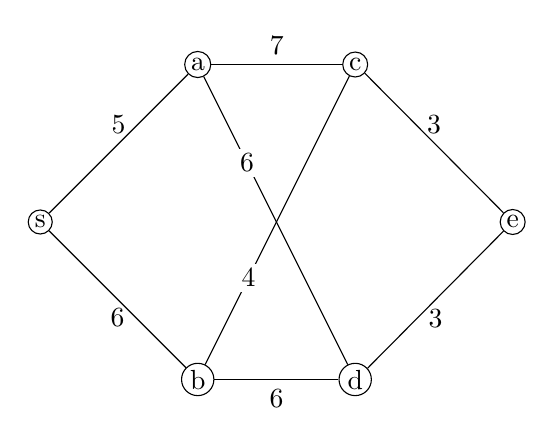
\begin{tikzpicture}[scale=2]
\node[draw,circle, inner sep=1pt](s) at (0,0){s};
\node[draw,circle, inner sep=1pt](a) at (1,1){a};
\node[draw,circle, inner sep=1pt](b) at (1,-1){b};
\node[draw,circle, inner sep=1pt](c) at (2,1){c};
\node[draw,circle, inner sep=1pt](d) at (2,-1){d};
\node[draw,circle, inner sep=1pt](e) at (3,0){e};
\draw (s) -- (a) node [midway,above]{5};
\draw (s) -- (b) node [midway,below]{6};
\draw (a) -- (c) node [midway,above]{7};
\draw (a) -- (d) node [pos = .3, inner sep = 2pt, fill = white]{6};
\draw (b) -- (c) node [pos = .3, inner sep = 2pt, fill = white]{4};
\draw (b) -- (d) node [midway,below]{6};
\draw (d) -- (e) node [midway,below]{3};
\draw (c) -- (e) node [midway,above]{3};
\end{tikzpicture}
\end{minipage}
%%%%%%%
\begin{minipage}[t]{.5\linewidth}
\begin{tabular}{ c | c | p{2in}}
Explored? & vertices & tentative distances\\ \hline
& \\
& \\
& \\& \\& \\& \\& \\& \\& \\% \\& \\& \\
 \end{tabular}

 \end{minipage}
 
 \vspace{1cm}

 
 \begin{tabular}{ c | c }
 vertex & minimum distance to s\\ \hline
& \\
& \\
& \\& \\& \\& \\& \\& \\& \\% \\& \\& \\
 \end{tabular}
\vfill
Think of an application of Dijkstra's Algorithm.
\end{document}